\section{Modello Concettuale}
Nel modello concettuale il sistema viene descritto come un sistema di code
connesse tra loro (figura~\ref{conceptual}), di quest'ultimo si distinguono i
seguenti componenti:
\begin{itemize}
\item[\textbf{Cloudlet}:] nodo del sistema che comprende un numero $N$ di server
senza coda che operano in parallelo con tassi di servizio specifici per classi
di job.
\item[\textbf{Cloud}:] nodo del sistema che comprende un numero infinito di
server senza coda che operano in parallelo con tassi di servizio specifici per
classi di job.
\item[\textbf{Centro di setup}:] nodo del sistema che modella la fase di setup
di un job interrotto, composto da un numero infinito di server senza coda che
operano in parallelo con un tasso di servizio pari a $1/E[S_{setup}]$. Un job
interrotto transita per questo centro prima di prendere servizio nel cloud ed il
tempo ivi trascorso corrisponde al tempo necessario alla ri-esecuzione del job.
\item[\textbf{Controllore}:] componente che implementa la logica di routing in
base all’occupazione del cloudlet tenendo conto del parametro di soglia $S$, non
costituisce un centro di servizio in quanto la sua funzione è limitata
all'inoltro dei job.
\end{itemize} 
%
\begin{figure}[!h]
\centering
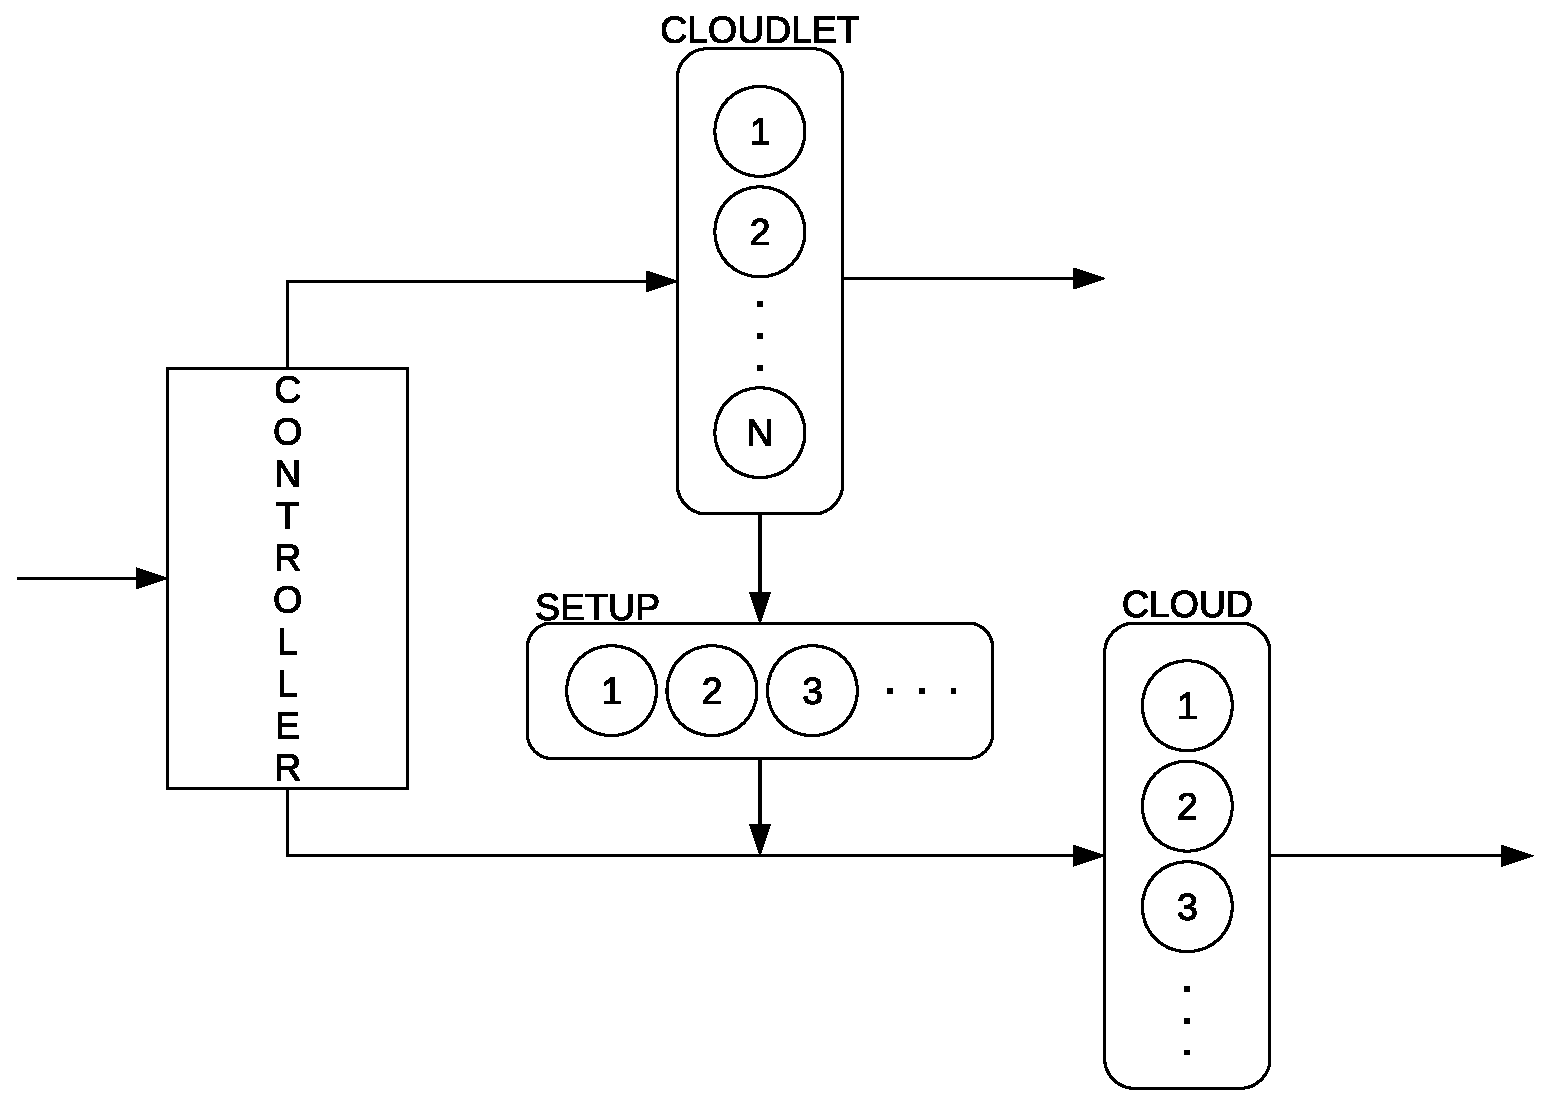
\includegraphics[width=0.7\textwidth]{figures/conceptual}
\caption{Modello concettuale del sistema}
\label{conceptual}
\end{figure}
%
Ogni job che arriva al sistema passa prima per il controllore, il quale decide
quale deve essere il nodo di esecuzione (cloud o cloudlet). Se arriva un job di
classe 1 ed il cloudlet si trova nella condizione per cui almeno un suo server
ha in esecuzione un job di classe 2 e la somma dei job presenti ha raggiunto il
valore di soglia $S$, allora tale server deve sospendere il job e sostituirlo con
quello appena arrivato di classe 1. Il job di classe 2 interrotto verrà poi
inoltrato al server remoto (cloud), non prima però di aver trascorso un tempo
necessario alla propria riesecuzione sul nuovo nodo, tale fase è modellata
assumendo che il job venga eseguito in un centro intermedio (centro di setup).
